\documentclass[12pt]{scrartcl}
\input{NiaLatexHelpers/nia_defs.tex}
\parskip=0.5cm

\title{\vspace{-2em}Functions and Debugging}
\author{}
\date{}
\begin{document}
\maketitle
\vspace{-6em}
\section*{Programming Functions Are Like Math Functions}
Think of math functions like $f(x) = 3x + 2$ or $f(x) = x^2$. We're often taught to see functions like machines that take inputs and churn out outputs.
\begin{figure}[H]
    \centering
    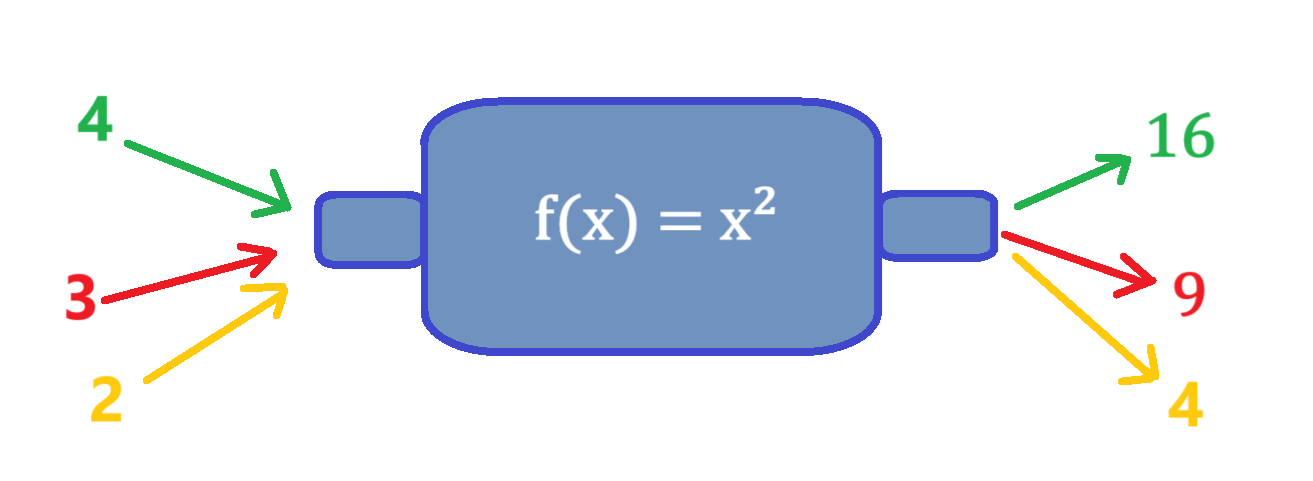
\includegraphics[scale=0.4]{Math Functions as Machines.png}
    \caption*[This function takes in numbers and sqaures them.]
\end{figure}
Programming functions are like that to! Imagine a function that takes in strings (English words) and adds an exclamation point to the end:
\begin{figure}[H]
    \centering
    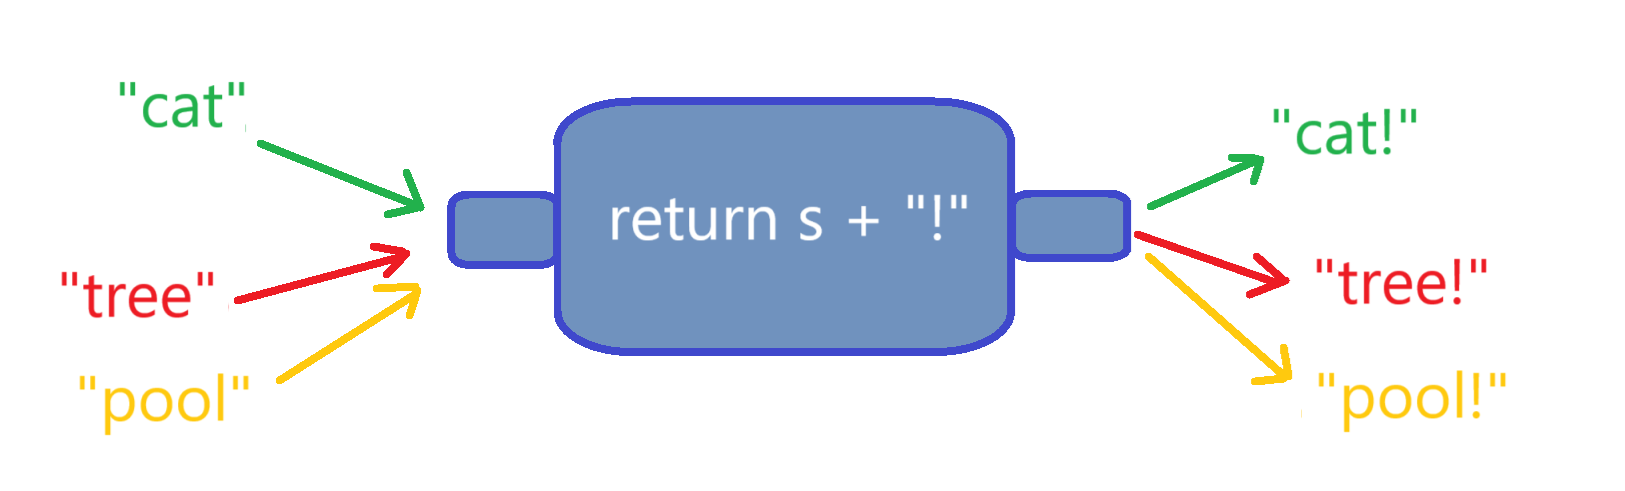
\includegraphics[scale=0.38]{CS Functions as Machines.png}
    \caption*[This function takes in strings and adds an exclamation point to the end.]
\end{figure}

\end{document}